\documentclass[10pt,conference]{IEEEtran} 

\usepackage{latexsym,times}
\usepackage{epsfig}
\usepackage{amsmath}
\usepackage{graphicx,dblfloatfix}
\usepackage{tabularx}
\usepackage{verbatim}
\usepackage{listings}
\usepackage{algorithm}
\usepackage{algpseudocode}
\usepackage{caption}
\usepackage{multirow}
\usepackage{pifont}
\usepackage{balance}

%\setlength{\textwidth}{6.5in} \setlength{\textheight}{8.5in}
%\setlength{\columnsep}{2.0pc} \evensidemargin=0in
%\oddsidemargin=0in
%\renewcommand{\textfloatsep}{8pt}
%\topmargin=-0.43in \topskip=0pt
%\renewcommand{\textfraction}{0.0}
%\renewcommand{\topfraction}{1.0}
%\renewcommand{\dbltopfraction}{1.0}

%\def\denseitems{
%\itemsep1pt plus1pt minus1pt
%\parsep0pt plus0pt
%\parskip0pt\topsep0pt}


\newenvironment{smallitem}{
   \setlength{\topsep}{0pt}
   \setlength{\partopsep}{0pt}
   \setlength{\parskip}{0pt}
   \begin{itemize}
   \setlength{\leftmargin}{.2in}
   \setlength{\parsep}{0pt}
   \setlength{\parskip}{0pt}
   \setlength{\itemsep}{0pt}}{\end{itemize}}

\newenvironment{smallenum}{
   \setlength{\topsep}{0pt}
   \setlength{\partopsep}{0pt}
   \setlength{\parskip}{0pt}
   \begin{enumerate}
   \setlength{\leftmargin}{.2in}
   \setlength{\parsep}{0pt}
   \setlength{\parskip}{0pt}
   \setlength{\itemsep}{0pt}}{\end{enumerate}}

\newenvironment{smalldescription}{
   \setlength{\topsep}{0pt}
   \setlength{\partopsep}{0pt}
   \setlength{\parskip}{0pt}
   \begin{description}
   \setlength{\leftmargin}{.2in}
   \setlength{\parsep}{0pt}
   \setlength{\parskip}{0pt}
   \setlength{\itemsep}{0pt}}{\end{description}}

%\newcommand{\comment}[1]{{\sf (#1)}}
\newcommand{\equationstart}{\small
\abovedisplayskip=2pt \belowdisplayskip=2pt
\abovedisplayshortskip=6pt \belowdisplayshortskip=6pt}

\newcommand{\equationend}{\normalsize}

\begin{document}

\input{epsf}

\pagestyle{plain}

 \title{A Collaborative Filtering Recommender System \\ 
for Test Case Prioritization in Web Applications}

%\numberofauthors{2}
%\author{\IEEEauthorblockN{Author 1}
%	\IEEEauthorblockA{Departemant of ABC\\
%		University of x\\
%		X@ABC.edu}
%	\and
%	\IEEEauthorblockN{Author 2}
%	\IEEEauthorblockA{Departemant of ABC\\
%		University of x\\
%		X@ABC.edu}
%}

%\author{
%	\alignauthor Author 1\\
%	\affaddr{University of ABC}\\
%	\affaddr{x, y}\\
%	\email{authore1@abc.edu}
%	\and  % use '\and' if you need 'another row' of author names
%	% 4th. author
%	\alignauthor Author 2\\
%	\affaddr{University of ABC}\\
%	\affaddr{x, y}\\
%	\email{authore2@abc.edu}
%}

%\author{
%Maral Azizi \\
%University of North Texas\\
%maralazizi@my.unt.edu
%\and 
%Hyunsook Do \\
%University of North Texas \\
%hyunsook.do@unt.edu
%}

\maketitle
\thispagestyle{empty}


\begin{abstract}
The use of relevant metrics of software systems could improve
various software engineering tasks, but identifying relationships among
metrics is not simple and can be very time consuming. 
Recommender systems can help with this decision-making process; many applications
have utilized these systems to improve the performance of their applications.
To investigate the potential benefits of recommender systems in regression 
testing, we implemented an item-based collaborative filtering recommender
system that uses user interaction data and application change history 
information to develop a test case prioritization technique.
To evaluate our approach, we performed an empirical study using three 
applications with multiple versions and compared five control techniques.
Our results indicate that our recommender system can help improve the 
effectiveness of test prioritization; the performance of our approach
was particularly  noteworthy when we were under a time constraint.  
\end{abstract}



%\vspace*{6pt}
\textbf{Keywords: }{Recommender system, test case prioritization, 
regression testing, risk measurement, code quality.}

%\vspace*{12pt}
%
%\baselineskip=18pt

\section{Introduction}
\label{sec:introduction}
% what is the problem?
During application's life it may change several times, and one change can affect the entire system.
To avoid the undesirable change or bugs, system testers need to  
test the overall functionality of the system before deploy the new release of the system.
One of the most common way to evaluate the system quality in sequence of release is regression testing.
In regression testing, testers check the software to ensure that new changes have not 
introduced new faults or it did not effect the other parts of system.
Applying regression testing before deploying new release of the software, make the 
change process safer and more confident for developers.

As software grow, the size of test suite grow in a same
manner, eventually testing the entire system can become expensive and may take
40\% of whole project budget[].  Moreover, it is not feasible to test every single 
function of the system especially for large scale systems it may takes several days 
to execute test cases. Several techniques have been proposed to solve this issue 
%by reducing the cost and effort of system testing.
such as, test reduction which is a 
technique that select subset of test cases that can address most of the issues, 
test selection also is a similar to test reduction but the main difference is 
this technique, select test cases based on their correlation with the changes 
in tow versions of the subject, and test case prioritization [].

% what approaches have been proposed?
Test case prioritization is a technique to catch the faults earlier, 
by executing the most important test cases first.
So far, many prioritization strategies have been proposed by researchers [] and
many techniques have been purposed such as : greedy techniques [], change impact analysis [],
clustering approaches[], user session based techniques [], etc. 
but most of the investigated studies are based on two main features: code coverage and 
code complexity metrics. Meanwhile, there are many other features of the software 
that can be a factor of failure or can be a hint to find the failure causes. 
One interesting feature of web application is that recording users interaction data
is a way easier compare to other types of applications. 
Different types of data from users interaction can be
monitored, such as users sessions, cookies, telemetry data, users IP address etc. 
Storing and collection log files and users sessions nowadays are less costly and more 
accessible compare to past decades, due to lower price of the IT services and hardware.
We can store information in database or cloud system 
rather than log files which was a traditional way to storing system back up. 
Having all these types of data and facilities, enables testers to identify most frequently used
components which impact the system strongly. 
% jeff paper

% why they didint work?
Previous studies shown that change history has more significant role in 
terms of finding faults than code metrics []. 
Although, there are several research have been done about the efficiency of 
change metrics for defect prediction, such as [] but, researchers only focused on 
measuring the causes and effect of the changes in software. 
Moreover, users session and telemetry data 
have been used as a factor for research in software testing. 
For example, Elbaum et al.~\cite{elbaum2005profiling} performed a study on regression 
prioritization focusing prioritization at a product level 
by using telemetry from installations. 
Their work was extended in several domain such as, performance issue detection ~\cite{parsons2007automatic},
bug detection ~\cite{wang2008approach}, reliability testing of rule-based 
systems ~\cite{avritzer1996reliability} and failure reproduction ~\cite{jin2012bugredux}. 
Sampath et al. ~\cite{Sampath2008} applied multiple techniques for prioritizing test cases 
by using user sessions as a factor for their techniques. 


Lets conciser a typical test prioritization based on change history. 
In this scenario, testing is based on executing any component that has been 
changed in new release of software [1-2], % ref: A Comparison of Coverage-Based and Distribution-Based Techniques for Filtering and Prioritizing Test Cases
while this could be a minor change that 
does not have a considerable impact on the entire system, 
such as renaming a function or can be a 
component that is used seldom by users, etc. 
In another scenario, we reorder test cases based on the component frequency, 
meanwhile, there might be no change in this particular component compare to previous version.
For example, generally, core components in a system are mostly used components in the entire system 
while, those components due to their significant role have been tested several times and rarely change. 
Due to above challenges, we belive that current studies in test prioritization 
is neither efficient nor sufficient to address the test priritization problem. 
%We believe that applying multiple factors
%rather than focusing on a specific viewpoint would help improve test case prioritization techniques.

%such as, extracting usage patterns from telemetry data besides analysis of change history. 


% what is your solution and why this work?
In this paper we proposed an item based collaborative filtering recommender system 
for test case prioritization in web application which, uses the telemetry 
data as input for users rating and change history of applications 
as items information. The output of our recommender system is the prioritized test 
cases in a way to obtain the better results in terms of finding faults earlier. 
We applied our recommender system in three open source system and one commercial system.
Our hypothesis is: Combination of various metrics can lead us to design 
more efficient model for fault detection. Our approach focuses on both users 
interaction and change history metrics to detect most risky components, then by 
automating the detection of regression issues, we are reducing the analysis effort for 
test prioritization. Our recommender system, may not locate the regression issue sources 
directly, but it will provide a  list of top potential risky components. 

The main contributions of this study are as follows:
1) Proposing a new hybrid test prioritization technique for web applications domain, 
2) Empirical evaluation of proposed technique and three other control techniques, and
3) Highlighting issues occurred during applying the proposed technique and its limitation 
and guidance to testers upon the results of our study. 

The rest of the paper is organized as follows. In Section 2, we
discuss the approach used in the research as well as formally define
collaborative filtering recommender systems. In Section 3, we detail the empirical study
that we performed. Section 4 provides the results of the study. 
Section 5 discusses the results and the implications of these results, and
Section 7 presents related work. Finally, in Section 8, we provide
conclusions and discuss future work.




%The usage of web application in nowadays is very clear for verity of people 
%from IT expert to someone with minimum knowledge of the Internet. 
%Not only many business are dependent on web applications but also
%web application grow very fast, and number of users of web application are
%growing exponentially, these factor made software engineer to spend 
%more time on deign robust system with minimum failure risk. 
%One small bug can cost so much money and time for the company.
%So far many research have been done to eliminate the risk of
%web applications failure such as test driven development, regression testing, 
%and many more but they are not sufficient neither optimum to detect the faults 
%when it occurs. 
%
%During application life it may change several times, and one change can affect the entire system.
%To avoid the undesirable change or bugs, system testers need to  
%test the overall functionality of the system before deploy the new release of the system.
%But still there might be some issues that can be observe later after deployment.
%One of the most common way to evaluate the system quality is regression testing.
%In regression testing, tester are seeking to find the cause of system failure 
%between old and new versions. Advantage of regression testing is, it make the 
%change process safer and more confident for developers.
%By fast increasing size of software systems, 
%size of test suits grow exponentially as a result, testing the whole system is a time consuming process 
%and can take several days, also it is not feasible to test every function of the system.
%Test case prioritization is 
%a technique to catch the faults earlier, by executing the most important test cases first.
%There are different ways to reorder test cases such as code coverage based, 
%based on frequency of use, based on system architecture and many other statistical technique [xx].
%
%
%Another feature of web applications which made it more popular
%compare to other types of software systems is users monitoring and recording 
%users activity is a way easier and accessible [bryce and others]. 
%% example of ppl who used telemetry
%% and converting usage
%There are different types of data from users interaction can be
%monitored, such as users sessions, cookies, telemetry data, users IP address etc. 
%having all these information has several benefits but to mention the most significant in testing area is that it gives an opportunity to the system tester
%to extract the pattern of most frequently used components of the system so, they can spend more effort 
%of fixing issues of such a components than others.
%
%In this paper we proposed a collaborative filtering recommender system 
%for test case prioritization in web application which, uses the telemetry 
%data as input data of users interaction and change history of applications 
%as items information. The output of our recommender system is the prioritized test 
%cases in a way to obtain the better results in terms of finding faults earlier. 
%We apply our recommender system in three open source system and one commercial system.
%
%The rest of the paper is organized as follows. In Section 2, we
%discuss the approach used in the research as well as formally define
%telemetry fingerprinting. In Section 3, we detail the empirical study
%that we performed. Section 4 provides the results of the study. 
%Section 5 discusses the results and the implications of these results, and
%Section 7 presents related work. Finally, in Section 8, we provide
%conclusions and discuss future work.
%

















\section{The Proposed Approach}
\label{sec:approach}

In this section, we describe the proposed approach, which utilizes
an item-based recommender system to improve test case prioritization techniques. 
Figure~\ref{fig:workflow} shows three major activities in our approach and
how these activities are related to each other. 
The first step of our proposed technique is usage pattern extraction, 
which is shown in the upper box of the Figure~\ref{fig:workflow}. 
In this activity, we analyze the users' interaction data to 
determine the most frequently accessed components of the system. 
Our second activity is change history analysis, which is shown in the
lower box of the Figure~\ref{fig:workflow}. In this activity,  
we build a classification model to 
measure the relationship between software defects and change history metrics. 
Then, by obtaining the output from these two activities, we measure the risk 
score of each component and prioritize the test cases based on their coverage
of these risky components. In this paper, component refers to method. 

\begin{figure*}[!hb]
\vspace*{-12pt}
	\centering
	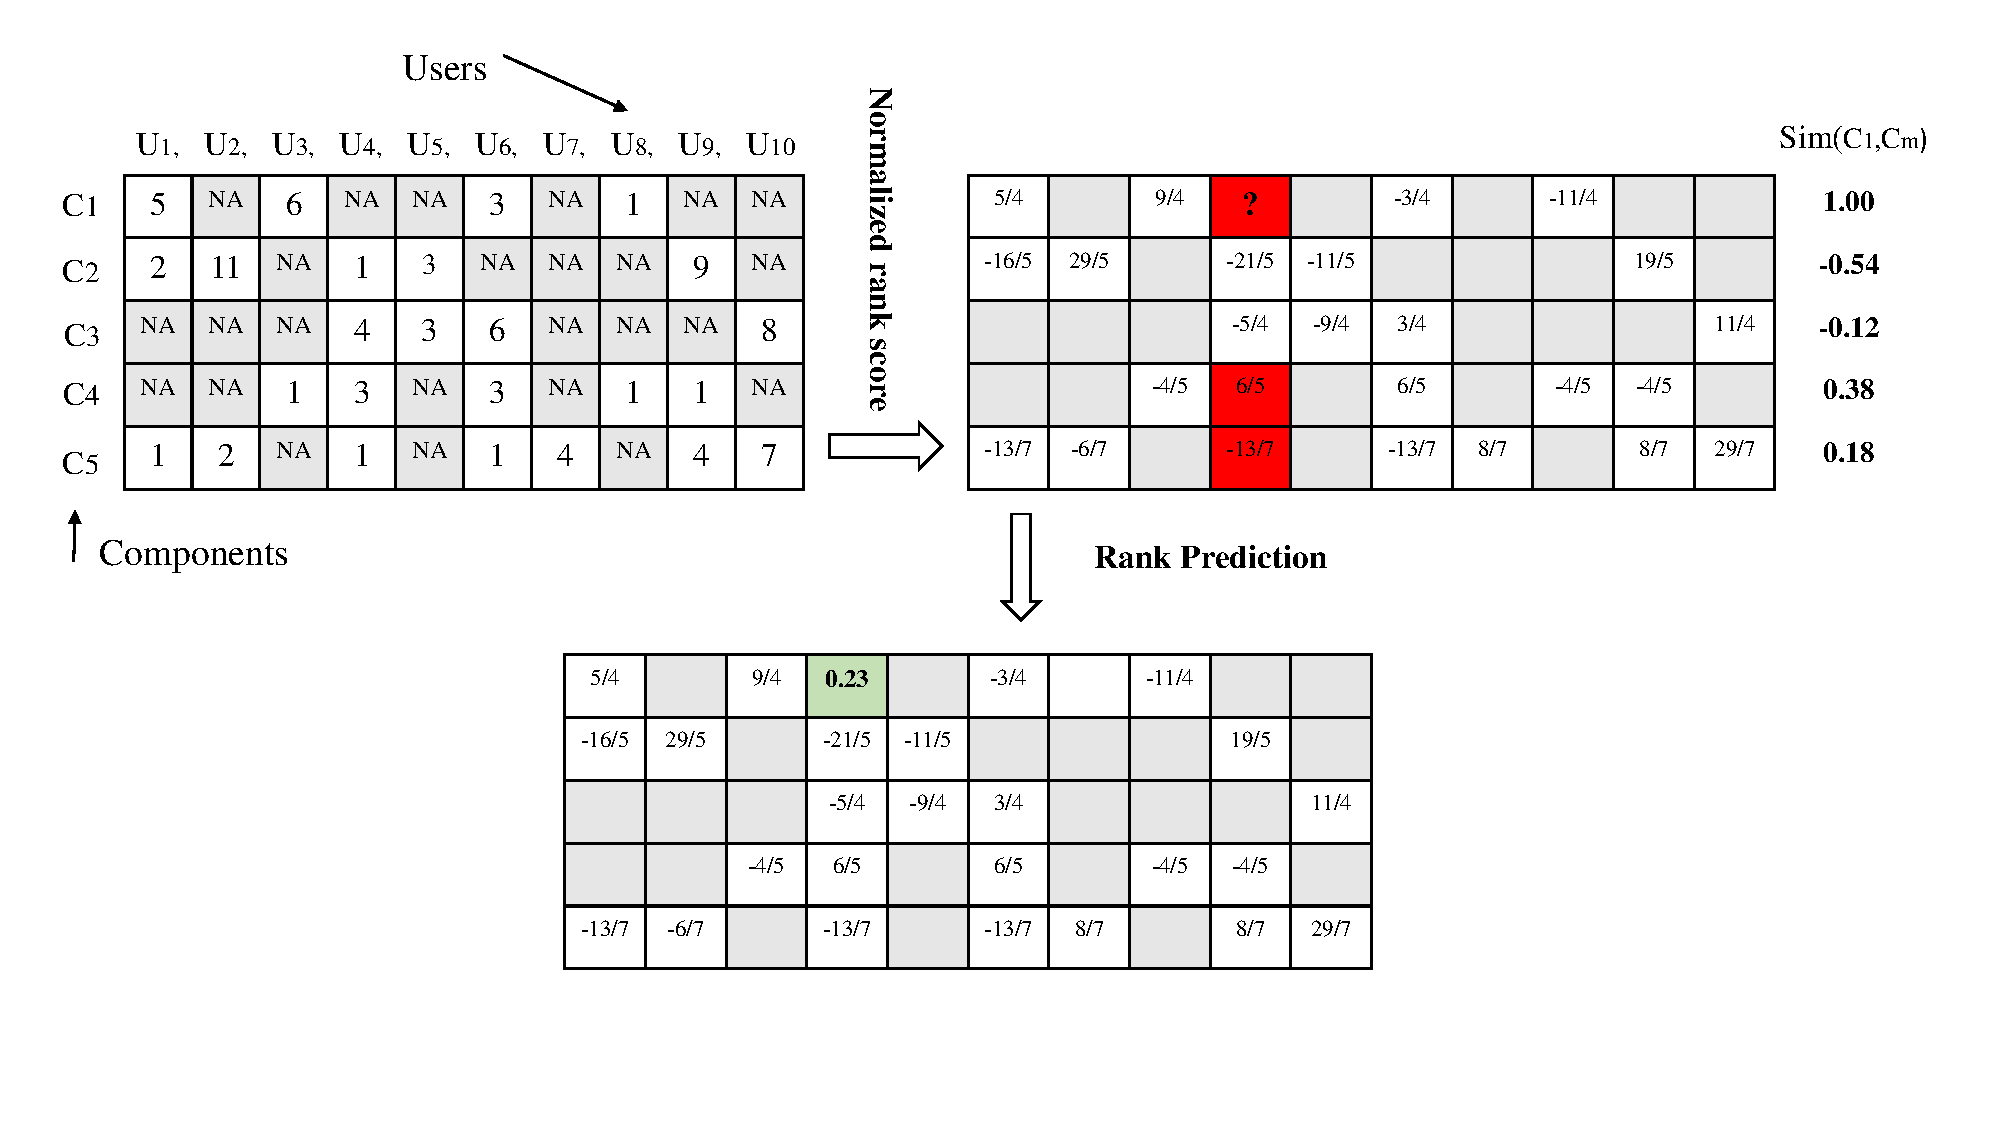
\includegraphics[width=0.8\linewidth]{./collaborative-filtring22.pdf}
\vspace*{-30pt}
	\caption{Item-Based Collaborative Filtering Process for Identifying Most-Frequent Components}
	\label{fig:collaborataivefiltering}
\end{figure*} 

\subsection{Usage Pattern Extraction}
\label{recommender-approach}

The goal of our recommender system is to suggest the highest-risk 
components with the most access frequency among all other components in the applications. 
In large scale applications, there are wide range of features and components; 
however, in reality, only a relatively small subset of components is accessed by users. 
Therefore, even if there are bugs in some part of the system that is not generally access by  users, we assume that those bugs have less impact on the user-reliability perception
of a system; catching those bugs that have been exposed by users is a bigger priority.
Also, prioritizing the test cases that exercise these more
frequently accessed components can speed up the rate of fault detection. 
 
There are two primary techniques for collaborative filtering algorithms:
user-based and item-based algorithms. 
A user-based collaboration filtering algorithm tries to find 
users who are most similar to the current active user.
In an item-based algorithm, first we design a model of user rating, 
and then we evaluate the expected ratings of an item based on the previous 
ratings of the other similar items. Because our concern is to find the 
access frequency of the components rather than user preferences, 
we chose an item-based algorithm.

To calculate the access frequency of the components,
we used two collected data sets: 
a list of users $U=\{u_1, u_2, ..., u_m\}$ and 
a list of the components $C =\{c_1, c_2, ..., c_n\}$. 
Each component $c_i$  has a list of users' ratings if 
users have performed at least one task with it.
Typically, in recommender systems, prediction is based on the numerical values of 
ratings from active users, but in our case we do not have access to such rating 
modules; instead, we refer the value of access frequency for a specific component 
by an individual active user as a rating score. 

Suppose that a user has interacted with a set of components,
$\{c_1, c_2,$ $..., c_n\}$. 
The item-based collaborative algorithm
computes the similarity between components by calculating the cosine similarity 
of the ratings of two components. 
Then, the algorithm selects the $N$ most similar components 
%$\{c_1, c_2, ..., c_N\}$ 
that has the highest similarity score to $c_i$.
%We defined the set of $k$ most similar components as $N$.
%Further, corresponding similarities $\{s_{i1}, s_{i2}, ..., s_{ik}\}$  
%between components are also estimated. 

After finding the components that have the highest similarity score, 
we need to predict the ratings of those
components that have been ignored or have not yet been used.
To do this, the algorithm uses a weighted average of the target user ratings
on these similar components.
Below, we describe the process of computing similarity and ranking.

Suppose that we have a web application that has several functionalities; 
a group of users shows similar interests in using a set of components,
while other groups of users use different sets of components. 
We want to measure the similarity between components by considering users' activities 
and their preferences in using the components.
 
Figure~\ref{fig:collaborataivefiltering} illustrates an example of
component similarity prediction. The upper left-hand matrix in the figure shows 
how many times each component has been used by users. 
The numbers in the cells show the access frequency by the
user $u_{i}$ on the component $c_{j}$, 
and $NA$ indicates that the user $u_{i}$ has not used that 
particular component yet. In this figure, $u_{1}$, $u_{3}$, $u_{6}$, and $u_{8}$ 
utilized components $c_{1}$; and $u_{1}$, $u_{2}$, $u_{4}$, $u_{5}$, and $u_{9}$ 
utilized $c_{2}$. 
We refer to a set of component ratings as a component vector.
For example, the vector $c_1$ is $\{5, NA, 6, NA, NA, 3, NA, 1, NA, NA\}$. 
Once we identify the component vectors, we measure the similarity 
between $c_{i}$ and all other components one by one. 

In order to determine the similarity between two components $i$ and $j$, we use
Pearson-r correlation~\cite{recom}.
If $U$ is the set of users who rated components $i$ and $j$, then we compute
the correlation similarity using the following equation:

\vspace*{-3pt}
\[
{Sim (i,j) = \frac {\sum_{u\in {U}}(C_{u,i} - \bar{C_i})(C_{u,j} - \bar{C_j)}}
	{ \sqrt{\sum_{u\in {U}}({C_{u,i} - \bar{C_i}})^{2}}
		{ \sqrt{\sum_{u\in {U}}({C_{u,j} - \bar{C_j}})^{2}}}}}	
\]

where $C_{u,i}$ is the value of access frequency for component $i$ by user $u$, and
$\bar{C_i}$ is the average access frequency value of $C_i$ . 

The reason for finding the similarity between components is to find the missing 
value in the matrix. To measure the similarity between components, 
we normalize the rating of each component by subtracting the row mean. 
The upper right-hand matrix in Figure~\ref{fig:collaborataivefiltering} shows the normalized
rating values of the left matrix. 
For example, the average of access frequency of $c_{1}$ and $c_{2}$  is $15/4$ and $26/5$, respectively.
Then, we subtracted mean values from each corresponding row of the left matrix.  
Positive values indicate that the user liked the component more than average;
while negative values
indicate that the user liked the component less than average; 0 indicates the average access 
frequency for a component. 
We treat blank values as 0.
The rightmost column in the upper right-hand matrix shows the similarity 
between $c_{1}$ and all other
components. For example, $Sim(c_{1},c_{2})= -0.54 < Sim(c_{1},c_{4})= 0.38$ means
that the probability of rating of $c_{1}$ is much more like $c_{4}$ than $c_{2}$.  

After calculating the similarity between all components, we select 
the set of $N$ most similar components for $c_{i}$;  
this process will be iterated for every component. 
Once we have this set of $N$, then we can make a prediction of access frequency 
for the missing values of $c_{i}$ based on a rating of the $N$ similar components.
To estimate the access frequency rates of ignored components, we performed
ratio prediction computation using a weighted sum method.
This method provides the ratio prediction of a specific component $i$
for user $u$ based on similar components. 

\vspace*{-3pt}
\[
{P_{u,i} = \frac {\sum_{{all\: simillar\: components , N}}(S_{i,N} * R_{u,N})}
	{\sum_{{all\: simillar\: components, N}}({S_{i,N}})}}
\]

$R_{u,N}$ is the rating score for user $u$ and $N$ most similar components, 
and $S_{i,N}$ is the similarity score of component $i$ and $N$.

We illustrate this using an example in Figure~\ref{fig:collaborataivefiltering}.
The lower matrix in the figure shows the predicted frequency access for $P_{1,4}$, 
which is calculated by $(0.38 * 6/5 + 0.18 * -13/7) / (0.38 + 0.18) = 0.23$.   

The number, $N$, is determined based on the context of application domain, 
ranging from 1 to size of $C - 1$. 
However, assigning a large number to 
$N$ will increase the calculation cost significantly, while the result accuracy would not
change noticeably. Therefore, to reduce the cost of the calculation process, 
we set $N=2$ , 
which means that to predict the missing values we only
select the two most similar components to $c_i$. 
This process is repeated until we find the ranking for the all missing values. 
Once we calculate ratio scores for the components, we can produce a matrix of components
and their access frequency ranking scores.  
We calculate normalized access frequency scores
using the following equation:

\[
{F_{Ci} = \frac {{\sum}(P_{Ci})}
	{{number\: of\: components}}}
\]

where $P_{Ci}$ is the predicted rank score and $F_{Ci}$ is the
normalized rank score of component $i$. 
Then we can sort the matrix of components based on their ranking to 
select $Top-N$  most frequently accessed components.

\vspace*{-3pt}
\subsection{Change History Analysis}
\label{CIA-approach}
\vspace*{-2pt}

The second phase of our proposed approach is change history analysis.
Among hundreds of attributes of code and change history metrics to evaluate
the code quality and error proneness, we chose change history metrics to identify
the riskiest components. According to a previous study~\cite{raimund},
change history is a better indicator for bug prediction purposes than code metrics.
 

The process of change analysis involves two major steps. 
First, we collect change history information (e.g., added lines of code,
deleted lines of code, etc.) and bug reports
from all available versions of the
applications from their repositories.  
The details of collecting the change history information 
are discussed in Section~\ref{data-collection}.  
Once the change history data is collected, 
we then design a linear model from a set of collected 
change metrics to build a classification model for bug prediction.
Our goal is to find the correlation coefficient of each 
metric to measure statistical relationships between a change metric and 
real defects. 
The value of this measure 
ranges between 1 and -1, where 1 indicates a strong 
positive relationship, 0 indicates no correlation, and a
negative value indicates a reverse correlation.

To evaluate our linear model, we applied 10-fold cross validation
and repeated this process 100 times. 
We used a common accuracy indicator to determine the accuracy of 
our model. 
%Table~\ref{tab:ConfusionMatrix} shows the confusion matrix that we used
%for accuracy evaluation.
The three accuracy indicators that we used are PC, TP and FP. 
PC indicates the percentage of correctly classified 
instances,
% which is calculated using $(m_{11} + m_{22})/(m) * 100\% $. 
TP (true positive) indicates the number of components
that contain a bug (and our classification
model also classified them as buggy components), 
%which is obtained by $m_{22}/(m_{22} + m_{21})$,
and FP (false positive) is the number of components that 
are classified as buggy (but they are clean). 
%which is calculated by $m-{12}/(m_{12}+m_{11})$ . 
%A higher PC value means that our classifier model is effective. 
The output of our classification model is a list of components with
their risk values, $I_{Ci}$ (the risk score of being buggy for component $i$).

%\begin{table}[!ht]
%	\caption{Confusion Matrix}
%	\vspace*{-10pt}
%	\begin{center}
%		\begin{tabular}{|l||c||c||c|}
%			\hline
%			Metrics     & Predicted: No & Predicted: Yes &  \\ \hline
%			Actual: No  &     $m_{11}$ = 33   &     $m_{12}$ =  63   & $m_1$ = 96 \\ \hline
%			Actual: Yes &     $n_{21}$ = 54   &     $m_{22}$ =  46   & $m_2$ = 100 \\ \hline
%			&      87       &       109      & $m$ = 196 \\ \hline
%		\end{tabular}
%		\end {center}
%		\label{tab:ConfusionMatrix}
%		\vspace*{-5pt}
%\end{table}
	
%A higher PC value means that our classifier model is effective 
%If PC is high but the recall (TP) low, this means that our classifier 
%classified a large number of components as clean when they are not, 
%indicating that we missed many buggy component during this phase
%of testing. However, if FP is high, this indicates that our model detected many components as buggy when they 
%are clean, and this will add extra cost to test the system when such a cost is not warranted. 
%The output of our classification model is a list of components with
%their risk values, $I_{Ci}$ (the risk score of being buggy for component $i$).

\vspace*{-3pt}
\subsection{Test Prioritization Using the Recommender System}
\label{test-prioritization}

After obtaining the two metrics explained in previous subsections (component risk scores and 
access frequency ratios), we calculate the final risk scores using the following equation:

\vspace*{-3pt}
\[
{ R_{Ci} = F_{Ci} * I_{Ci}}	
\]

\vspace*{-3pt}
where $F_{Ci}$ is the access frequency score of component $i$ 
and $I_{Ci}$ is the fault risk score of $C_i$.  

Using $R_{Ci}$ scores, our recommender system provides a ranked list of components.
The ranked list of components contains those components of the system that are most
likely to be the cause of regression faults. 
As shown in Figure~\ref{fig:workflow}, the test case prioritization algorithm
reads two inputs (a recommended $Top-N$ list of components and code coverage of tests),
and reorders test cases. 

For example, suppose we have five components
$C =\{c_1, c_2, ... , c_5\}$ with risk scores 
$R =\{0.0014, 0.251, 0.034 , 0.561, 0.138\}$.
Also, suppose we have a list of test cases with their code coverage information
, such as $TC =\{T_1 ={(c_5, c_3)}, T_2={c_1}, T_3={(c_4, c_2)}, T_4={(c_2,c_5)} , T_5={c_2}\}$ .
Then, we reorder the test cases in this order:
$T_3, T_4, T_1, T_2, T_5$, 
since $T_3$ covers $c_4, c_2$, the two components 
having the highest risk score (0.561 + 0.251 = 0.812), and $T_2$ and $T_5$ will be
executed last because $T_2$ covers $c_1$, which has the lowest risk score (0.0014).
$T_5$ only covers $c_4$ (this component has been covered by $T_3$ as well); and because 
$T_4$  covers more components (0.251 + 0.138 = 0.389), then it has higher priority than 
$T_5$, which covers only $c_2 = 0.251$.
Finally, we calculate the fault detection rate of the reordered test cases by 
applying the proposed technique in the latest version of each application.  



\section{Study}
\label{sec:study}

Our study investigates whether the use of a recommender system 
can improve the effectiveness of test case prioritization techniques
considering the following research questions.

\begin{smallitem}
\item RQ1: Can our recommender system improve the effectiveness 
of test case prioritization techniques?

\item RQ2: Can our recommender system be effective in improving
the effectiveness of test case prioritization techniques 
when we have a limited time budget?
\end{smallitem}

The following subsections present our objects of analysis, 
study setup, threats to validity, and data analysis.

\subsection{Objects of Analysis}
\label{sec:objects}

To investigate our research questions, we performed an empirical study 
using two open source applications and one commercial web application.

\textbf{DASCP} is a digital archiving and scanning software designed for civil projects; 
we obtained this application from a private company.  
DASCP is a web based application written in ASP.Net and designed to store civil project 
contracts, which include the technical information of civil and construction projects 
such as project plans and relevant associated information. 
%DASCP includes an access control system and provides two types of access rights: 
%one user group has permission to edit or insert a project's information or 
%upload maps and contract sheets. The other user group is only allowed to view 
%the data and details about the projects.
Our second application is \textbf{nopCommerce}, which is a widely used open 
source e-commerce web application with more than 1.8 million 
downloads. This application is written in ASP.Net MVC and uses 
Microsoft SQL Server~\cite{nopCommerece}. 
The last application is \textbf{Coevery}, which is an open source 
customer relationship management (CRM) system written in ASP.Net. 
This application provides an easy framework for users to create their own customized 
modules without having to write any code~\cite{coevery}.
%The UI design of Coevery was developed 
%by AngularJS and Orchard Technologies~\cite{coevery}. 

\begin{table}
\caption{Application Properties}
\vspace*{-10pt}
\begin{center}
\begin{tabular}{|l|c|c|c|} \hline
\textbf{Metrics}  & \textbf{DASCP} & \textbf{nopCommerce} 
& \textbf{Coevery} \\\hline \hline
Classes   & 107  & 1,919& 2,258 \\\hline
Files  & 201  & 1,473 & 1,875 \\\hline
Functions & 940  & 21,057 & 13,041 \\\hline
LOC & 35,122 & 226,354 &120,897 \\\hline
Sessions  & 748 & 1310 & 274 \\\hline
Faults  & 35 & 70 & 30\\\hline
Versions  & 3 & 23 & 3 \\\hline
Test Cases & 95& 543 & 1,120 \\\hline
Installations & 3 & 2 & 1 \\\hline
\end{tabular}
\end {center}
\vspace*{-15pt}
\label{tab:AUTs}
\end{table}

Table~\ref{tab:AUTs} lists the applications under study and
their associated data: ``Classes'' (the number of class files), 
``Files'' (the number of files), ``Functions'' (the number of 
functions/methods), ``LOC'' (the number of lines of code), 
``Sessions'' (the number of user sessions that we collected), 
``Faults'' (the total number of seeded and real faults), ``Version'' (the number 
of versions), ``Test Cases'' (the number of test cases), and
``Installations'' (the number of different locations where the 
applications were installed). 
Test cases were in the application package; we did not generate any 
new test cases. We downloaded all available versions of open source applications 
from the applications' \textit{GitHub} repositories. 

\subsection{Variables and Measures}
\label{sec:measures}

\subsubsection{Independent Variable}

To investigate our research questions, we manipulated one independent 
variable: prioritization technique. 
We considered six different test case prioritization techniques,
which we classified into two groups: control and heuristic.
Table~\ref{tab:techniques} summarizes these groups and techniques.
The second column shows prioritization techniques for each group, 
and the third column is a short description of prioritization techniques. 

\begin{table*}[!ht]
\caption{Test Case Prioritization Techniques}
\vspace*{-10pt}
\begin{center}
\begin{tabular}{|l|l|l|}\hline
Group & Technique & Description \\ \hline
\multirow{4}{*}{Control} 
& Change history-based ($T_{ch}$) & Test case prioritization based on change risk analysis score.\\
& Most frequent web forms-based ($T_{mfw}$)&  Test case prioritization based on value of access frequency for each web form.\\
& Most frequent methods-based ($T_{mfm}$) &  Test case prioritization based on value of access frequency for each method.\\
& Random ($T_{r}$) &  Test case prioritization in random order.\\	
& Greedy ($T_{g}$) &  Test case prioritization based on the code coverage.\\\hline			
\multirow{1}{*}{Heuristic} 
& Hybrid collaborative filtering-based ($T_{hcf}$)& Test case prioritization based on the proposed technique. \\\hline
\end{tabular}
\end {center}
\label{tab:techniques}
\vspace*{-10pt}
\end{table*}

As shown in Table~\ref{tab:techniques}, we considered five control techniques and 
one heuristic technique. For our heuristic technique, we used the approach 
explained in Section~\ref{sec:approach},
so, here, we only explain the control techniques we applied as follows:

\subsubsection*{Change History-Based ($T_{ch}$)}
The first control technique is test case prioritization based on change risk
score. In order to perform this technique, we used the information that
we obtained from the change history analysis approach, which we explained in 
Section ~\ref{CIA-approach}. We prioritized our test cases based on the 
highest scores of the change risk list. 
	
\subsubsection*{Most Frequent Web Forms-Based ($T_{mfw}$)}
This approach determines the web forms that have been most frequently used by users. 
We assume that the most frequently used web forms play a more important role in the system; 
therefor, they should have a higher priority to be tested first. Another reason
why the access frequency of web forms is the key for testing is that the most frequently 
used web forms usually contain more functionality and links with other forms, 
so any bugs on those forms can affect a greater portion of the entire system. 
Here, we define ``base session'' as a long session performed by our users 
that displays the most interactions in the application ~\cite{jeff16}.
We picked 20\% of our total sessions as base sessions. 
For example, in online shopping, our base session is a sequence of actions
from user login to checkout, including all mandatory actions (e.g., payment) and some 
non mandatory actions such as browsing for other items, 
and checking the inbox during the shopping process.
	
\begin{figure}[!ht]
\vspace*{-3pt}
	\centering
	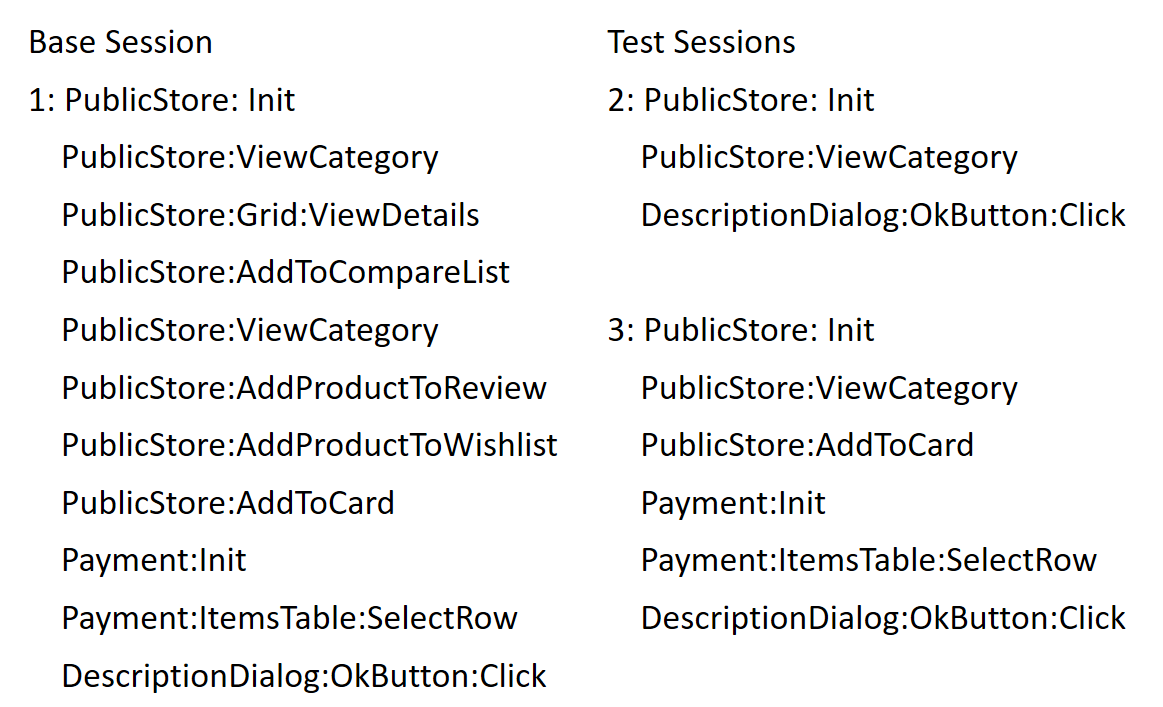
\includegraphics[width=0.90\linewidth]{./SessionSample4.png}
	\caption{Sample of Base Session and Test Sessions}
	\label{fig:sessions}
\end{figure}
	
After collecting all sessions, we conducted an analysis of web forms' access frequency 
by comparing the observed web forms in each session with a base session. 
	
\vspace*{-3pt}
\[
{F_{w,i} = \frac {\sum_{{form\: score\: for \: each\: session}}(S_{i})}
	{\sum_{{number \: of \: base \: sessions}}({BS_{i}})}}	
\]
	
Using Figure~\ref{fig:sessions} as an example, the form ``PublicStore'' 
from the base session was observed in test sessions 2 and 3. 
If we assume that we have ten test sessions and three base sessions,
and this particular form was observed in seven of the ten forms, then the
access frequency of form ``PublicStore'' is equal to $(0.7 / 3) = 0.23$.
	
\subsubsection*{Most Frequent Methods-Based ($T_{mfm}$)}
The most frequent methods approach is nearly identical to the web form frequency technique. 
The only difference is that we considered a method instead of a web form 
as a comparison factor. 
The most frequent methods usually have high dependency on other classes and methods. 
If one of them fails, it can cause a significant failure or degradation of the system. 
In order to prevent a domino effect in the system, high-frequency methods 
should be tested first, because their failure can cause 
other components to fail due to their dependencies.	 	

\subsubsection*{Random ($T_{r}$)}
The random prioritization technique randomly reorders test cases.

\subsubsection*{Greedy ($T_{g}$)}
The greedy technique reorders test cases based on the total number of 
blocks covered by test cases. 

\subsubsection{Dependent Variable} 

Our dependent variable RQ1 is the average percentage of fault detection (APFD)
referring to the average percentage of faults detected during the test suite execution. 
The range of APFD is from 0 to 100, the higher value indicating better prioritization technique. 
Given $T$ as a test suite with $n$ test cases and $m$ number of faults, 
$F$ as a collection of detected faults by $T$, and
$TF_{i}$ as the first test case that catches the fault $i$, 
we calculate APFD ~\cite{apfd} as follows:

\vspace*{-5pt}
%{\scriptsize
\[
{APFD = 1- \frac {{TF_{1} + TF_{2} + ... + TF_{m}}} {nm} + \frac{1}{2n}}
\]
%}
%\vspace*{-5pt}
	
RQ2 seeks to measure the effectiveness of our proposed approach
when we have constrained resources, which means that we need to evaluate 
the effectiveness of our approach using a different metric. 
Qu et al.~\cite{myra} defined the normalized metric of APFD, which is the
area under the curve when the numbers of test cases or faults are not consistent. 
The NAPFD formula is as follows:
	
\vspace*{-5pt}
%{\scriptsize
\[
{NAPFD = p- \frac {{TF_{1} + TF_{2} + ... + TF_{m}}} {nm} + \frac{p}{2n}}
\]
%}
%\vspace*{-5pt}
	
In this formula, $n$ is a percentage of the test suite run, 
$m$ represents the total number of faults found by all test cases,
$TF_{i}$ indicates the same parameter as AFPF, and 
$p$ is the number of faults detected by the percentage of our
budget divided by the total number of detected faults when 
running 100\% of test cases.  

%When evaluating RQ3, the primary concern is how fast test cases reordered 
%by our recommender system can detect all defects in the applications.
%The dependent variable for RQ3 is the total test execution time
%until 100\% defects are detected by each technique.  

\subsection{Data Collection and Experimental Setup}
\label{data-collection}
In order to perform our experiment, for both the control and heuristic techniques
we needed to collect three different types of datasets: telemetry data, change 
history, and code coverage information. We explain the data collection processes
in the following subsections.

\subsubsection{Collection of Telemetry Data}
To collect telemetry data, we implemented a small function to record user interactions. 
We considered a sequence of each user's interactions on a specific date as a user session.
First, we uploaded two applications, {\em Coevery} and {\em nopCommerce}, on an IIS server 
at the University of ABC in November 2016. 
The server specification is CPU Core i7, with 16 GB of RAM.
After deploying our applications, we recruited volunteer graduate and undergraduate
computer science students and assigned a variety of tasks to them. 
These tasks to the volunteers were simple scenarios that each application is designed for.
%%%%%%%% nemidoonammmmmmmmmmmmmmmmmmmmmmmmmmm
For example, in {\em nopCommerce}, we asked the volunteers to perform online shopping 
following the actual necessary steps, from login to payment. We also asked some of 
the users to be the system administrator, so we could monitor the whole system 
rather than only the end user side.
We asked the end users to access other part of the system randomly, for example,
checking their inbox or wish list.  
In total, seventy volunteer students performed different tasks during a forty-day period.  
%%% revierw question
We collected 1,310 and 274 user sessions for {\em nopCommerce}, 
and {\em Coevery} respectively. 
%%%%
 
The data collection process for {\em DASCP} is different from that of {\em Coevery} 
and {\em nopCommerce}. {\em DASCP} is a commercial and closed source application 
that has three versions, and it has been installed on the servers of three companies since 2011. 
The DASCP users whose data we examined are real users, and they have application domain knowledge.
We collected a twelve-month period of user interactions for DASCP.
As described in Section~\ref{sec:objects}, DASCP provides two types of access rights for users.
In this study, we only considered the sessions of those users who have full access to the system.
In total, 748 user sessions were collected during the designated period of time. 

%%% more details about sessions
However, the length of the sessions varied by user, date, and workplace.
For example, some users performed all their assigned task a few hours before the
determined deadline, while others distributed their tasks over several days.
The average length of user sessions for {\em nopCommerce} is equal to 56 and, for
{\em Coevery}, 24. However, in some case we obtained session lengths over 
300, especially when the interaction date was close to the deadline. 
Also, most of the {\em Coevery} users were selected among graduate students, since the
functionality of this application is relatively more complex that of {\em nopCommerce}. 

Figure~\ref{fig:SampleSession3} shows an example of the raw telemetry data. 
The left-hand column shows the session identifier, which is a user
navigating through the system. The right-hand column is the set of server-side user 
interactions. The structure of the interactions is of the format (Form name):(Control name):(Action name).

\begin{figure}[!ht]
\vspace*{-3pt}
	\centering
	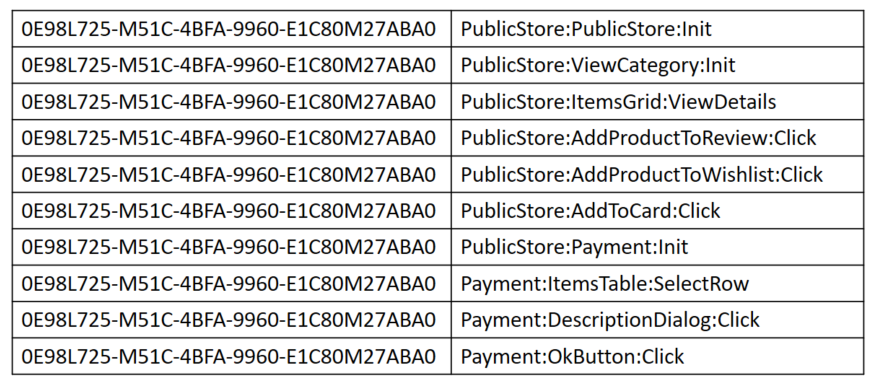
\includegraphics[width=0.90\linewidth]{./SessionSample3.png}
	\caption{Sample User Session}
	\label{fig:SampleSession3}
\end{figure}


\subsubsection{Collection of Code Change History}
We had to take three steps to measure change risk. 
First, we needed a clear understanding of the applications with respect to their changes.
For instance, we needed to check whether a change 
was just the renaming a variable or component, the addition of some comments, 
or an alteration of code by adding or deleting functions, and so on. 
Then, we needed to check whether changes had been made in the current version, 
and finally, we tested a recently changed system~\cite{change3}. 
%In order to collect change history information for training, 
%we used 23 versions of {\em nopCommerece}  and all available versions 
%of our two other applications. 
Figure~\ref{fig:versions} shows the versions that we used in this study. 
%%%%%% not sureeeeeeeeee
{\em nopCommerece} contains 36 versions but we used only the
versions available on the ~\textit{GitHub} repository as of the experiment date. However, for
{\em Coevery} and {\em DASCP}, we used all available versions. 
All studied applications contain fine-grained changes, and the commits on these two open source
applications are available in the \textit{GitHub} repository.   

\begin{figure}[!ht]
	\centering
	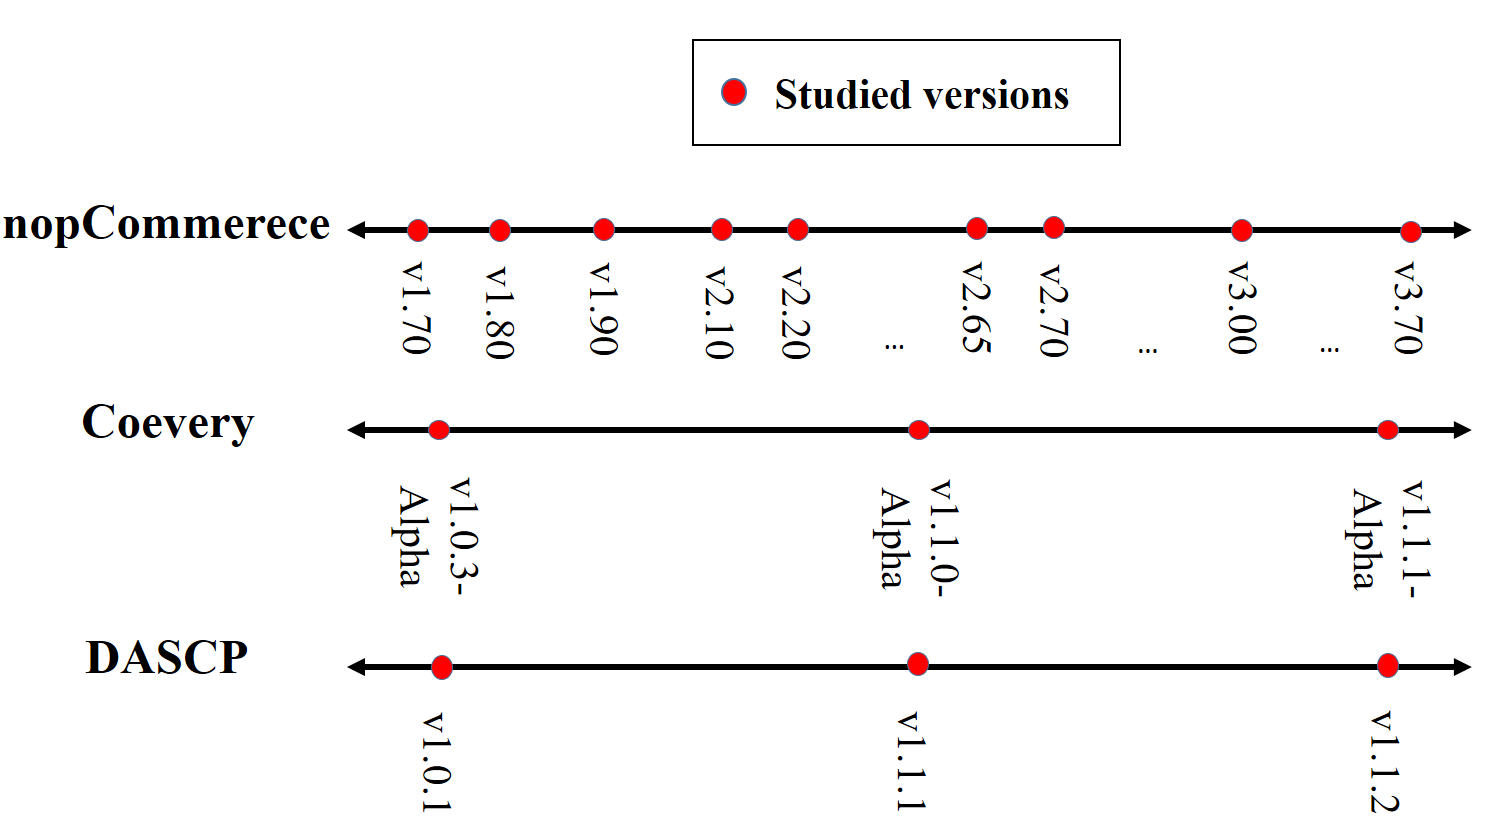
\includegraphics[width=0.95\linewidth]{./Versions2.png}
	\vspace*{-7pt}
	\caption{Versions of Each Application with Change Information and Bug Reports}
	\label{fig:versions}
%	\vspace*{-10pt}
\end{figure}\textbf{}

In our study, we collected the change history of our three applications 
following Giger et al.'s approach ~\cite{method}. 
%We chose ten metrics that have high correlations with bugs.
Most of these metrics have been used in bug detection research, and they
are known to be good indicators for locating bugs~\cite{sungmicro, shihab12, 
raimund, change1, change2, method}.
Table~\ref{tab:historyMetrics} shows the applied change metrics in this study. 

\begin{table}[!ht]
\caption{Change Metrics Used to Evaluate Risk}	
\vspace*{-3pt}
%\begin{tabular*} {.8\linewidth}{@{\extracolsep{\fill}}l|l|}
\begin{tabular} {|l|l|} \hline
	\textbf{Metrics Name} & \textbf{Description} \\\hline \hline
	Modification & Number of times a method was changed  \\\hline
	\multirow{2}{*}{LOC Added} & \parbox[t]{5.5cm}{Added lines of code to a  method \\ body over all method histories} \\\hline
	\multirow{2}{*}{Max LOC Added} & \parbox[t]{5.5cm}{Maximum added lines of code to a method \\ body for all method histories}\\\hline
	\multirow{2}{*}{AVE LOC Added}  & \parbox[t]{5.5cm}{Average added lines of code to a method \\ body per method history}\\\hline
	\multirow{2}{*}{LOC Deleted}  & \parbox[t]{5cm}{Deleted lines of code from a method \\ body over all method histories} \\\hline
	\multirow{2}{*}{Max LOC Deleted} & \parbox[t]{5cm}{Maximum deleted lines from a method \\ body for all method histories}\\\hline
	\multirow{2}{*}{AVE LOC Deleted} & \parbox[t]{5cm}{Average deleted lines from a method \\ body per method history}\\\hline
	Code Churn & Sum of all changes over all method histories\\\hline
	Max Code Churn & Maximum code churn for all method histories \\\hline
	AVE Code Churn & Average code churn  per method history\\\hline
	Age & \parbox[t]{5cm}{Age of a method in weeks from last release} \\\hline
\end{tabular}
\label{tab:historyMetrics}
\vspace*{-6pt}
\end{table}

\subsubsection{Collect Code Coverage}
\label{codecoverage}
Once our recommender system was designed and implemented, 
we needed to find test cases that covered the recommended components. 
We collected the code coverage data for our test cases using the code coverage analysis tool  
that Microsoft Visual Studio provides as part of its framework. 
After collecting the code coverage information, 
we entered it into a relational database. We assigned unique
identifier values for each method and test case, which provides
a key for method and test tables. Hence, we could easily map the methods
to the test cases that exercise them.  

 
\begin{table}[!ht]
\caption{Code Coverage Data Table}
\vspace*{-10pt}
\begin{center}
\begin{tabular}{|c|c|c|c|c|c|} \hline
	MethodID  & Risk Score & TestID1 & ... & TestID n \\\hline
	12 & 0.876 & 0 &  & 0 \\\hline
	287 & 0.012 & 1 &  & 0 \\\hline
	301 & 0.547 & 0 &  & 0 \\\hline
	148 & 0.145 & 0 &  & 1 \\\hline
	67 & 0.055 & 1 &  & 0 \\\hline			
\end{tabular}
\end {center}
\label{tab:coverage}
\vspace*{-10pt}
\end{table}

	
Table~\ref{tab:coverage} show the code coverage data we collected.
The first column, ``MethodID'', shows
the unique identifier values that we assigned for each method. 
The second column shows the final risk scores, which is the output of 
our recommender system. Other columns list our test cases
with Boolean values: 0 indicates that the test case does not cover 
the method, and 1 indicates that the test case covers the method.

\subsubsection{Faults}
\label{faultsInfo}

The applications contain real defects reported by users, but the number of 
defects is rather small considering the size of the applications we studied.
Thus, two graduate students seeded additional faults by simulating  programmers' 
common mistakes (e.g., using a single equal sign to check equality).
All seeded faults were in the server-side code level, and we ignored HTML-based and GUI faults. 
Four types of faults were seeded: (1) data faults that are related to interaction with 
the data store; (2) logic faults that are logic errors in the code; (3) action faults that modify 
parameter values and actions; and (4) linkage faults that change the hyperlinks references.  
Table~\ref{tab:AUTs} shows the total number of faults that including both real and 
seeded faults. The number of real faults for {\em nopCommerce}, {\em Coevery}, and 
{\em DASCP} is 25, 8, and 13, respectively. Once we collected all the required data, 
we ran control and heuristic 
techniques and calculated all the dependent values for the reordered test cases.


\section{Data and Analysis}
\label{sec:data}

In this section, we present the results of this study, considering
each of the two research questions. 

\subsection{RQ1 Analysis}

RQ1 investigates whether the use of the recommender system can 
improve the effectiveness of test case prioritization techniques.
%Figure~\ref{fig:All} shows the results combined for all applications.
Figure~\ref{fig:DASCP} presents the results for {\em DASCP}.
The vertical axis shows APFD scores, and the horizontal axis shows 
prioritization techniques:
``$T_{ch}$'' (change history-based), ``$T_{mfw}$'' (frequent web form-based), 
``$T_{mfm}$'' (frequent method-based), ``$T_{r}$'' (random order), 
``$T_{g}$'' (greedy technique), and 
``$T_{hcf}$'' (recommender system-based). 

\begin{figure}[!ht]
\vspace*{-10pt}
	\centering
	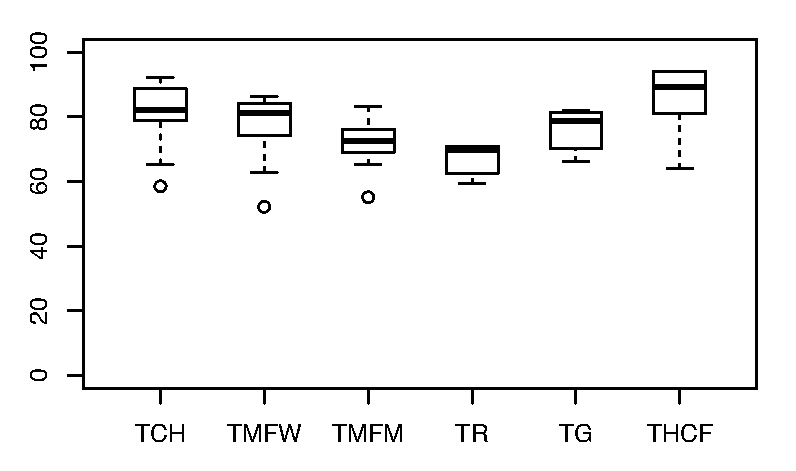
\includegraphics[width=0.90\linewidth]{./DASCPWGupdated.eps}
	\vspace*{-3pt}
	\caption{DASCP: APFD Boxplots}
	\label{fig:DASCP}
%\vspace*{-10pt}
\end{figure}

%Figure~\ref{fig:DASCP} presents the results for {\em DASCP}.
%Similar to the results that considered all applications, 
As can be seen the heuristic ($T_{hcf}$) outperformed all control techniques,
but data distribution patterns are different.  
%The variances are small, but there are more outliers.
Among control techniques, the random technique was 
the worst performer, whereas the frequent method-based technique ($T_{mfm}$)
produced results similar to the change history based technique ($T_{ch}$).


Figure~\ref{fig:nopCommerce} presents the results for {\em nopCommerce}.
The results show that our proposed technique outperformed  
all five control techniques, but the variance among the APFD scores is relatively high. 
Among the first three control techniques, the change history-based 
technique ($T_{ch}$) produced slightly better results than the others.
This application has 23 versions, and we had a sufficient
amount of change history data for our training, so we speculate that
this is the reason why the change history-based technique produced 
better results than the other control techniques. 
The greedy technique, which is the fifth control technique, did not yield 
better results than the other control techniques. 
The poor performance relative to other techniques could be explained by 
the nature of test cases of this application. A large number of test cases
have high code coverage, which caused the greedy technique which prioritizes based on 
block code coverage, to perform almost like the random technique.
 
\begin{figure}[!ht]
	\vspace*{-10pt}
	\centering
	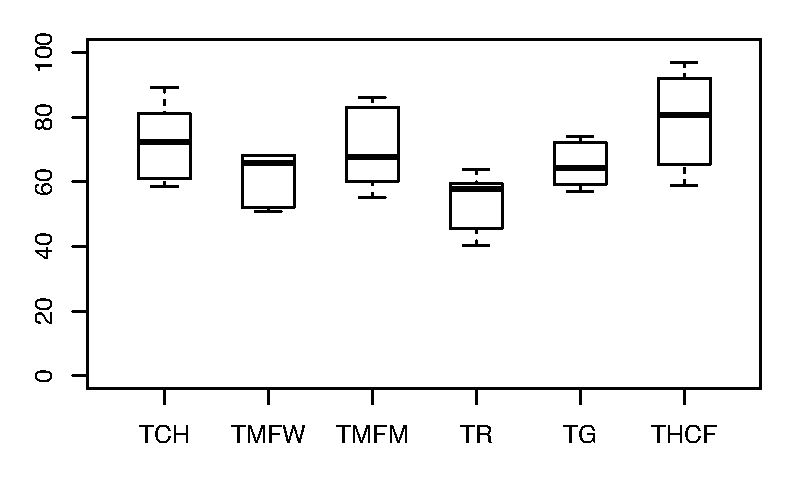
\includegraphics[width=0.90\linewidth]{./nopWG2updated.eps}
	\vspace*{-3pt}
	\caption{nopCommerce: APFD Boxplots}
	\label{fig:nopCommerce}
%\vspace*{-3pt}
\end{figure}

Figure~\ref{fig:Coevery} shows the results for {\em Coevery}. 
When we compared the median values, our heuristic technique improved
the rate of fault detection by 21\% over the four control techniques
($T_{ch}$, $T_{mfw}$ , $T_{mfm}$, and $T_{g}$) 
on average and 41\% over the random technique. 
Among the first three control techniques, $T_{ch}$ and $T_{mfw}$ 
produced slightly better results than $T_{mcf}$.

\begin{figure}[!ht]
	\vspace*{-10pt}
	\centering
	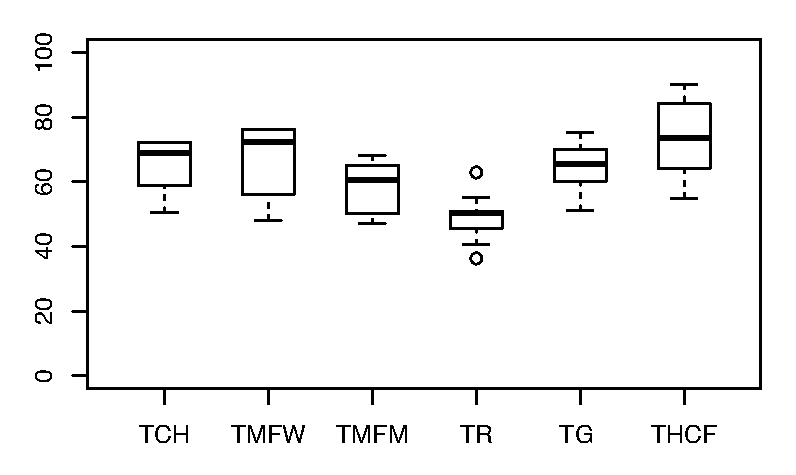
\includegraphics[width=0.90\linewidth]{./CoeveryWGupdated.eps}
	\vspace*{-3pt}
	\caption{Coevery: APFD Boxplots}
	\label{fig:Coevery}
%\vspace*{-10pt}
\end{figure}


Overall, the results showed that our proposed recommender 
system-based technique performed better than all the control techniques 
across all three applications. 
Among the control techniques, the random technique performed worst across all applications,
whereas the change history-based technique produced slightly better and more stable   
results for all applications.
Also, in the case of {\em DASCP} and {\em Coevery}, the greedy technique ($T_{g}$) 
showed marginally better results than other control techniques.

\begin{table*}[!ht]
\caption{NAPFD Scores on Average.}
\vspace*{-10pt}
\begin{center}
{\scriptsize
\begin{tabular}{|c|c|c|c|c|c|c||c|c|c|c|c|c|}\hline
Application & Test Exe. & \multicolumn{6}{c||} {Techniques} 
& \multicolumn{5}{c|} {Improvement Rate over Control} \\\hline \hline
& Rate (\%)  & $T_{ch}$ & $T_{mfw}$ & $T_{mfm}$ & $T_{r}$ & $T_{g}$ & $T_{hcf}$ 
& $T_{hcf}/T_{ch} $& $T_{hcf}/T_{mfw} $ & $T_{hcf}/T_{mfm}$ & $T_{hcf} /T_{r} $ &  $T_{hcf}/T_{g}$ \\\hline \hline
 
 
 &10	&18.54	&12.17	&15.12	&14.33	&16.53	&23.37	&26\%	&92\%	&54\%	&63\%	&41\%	\\
 &20	&21.31	&12.88	&16.78	&15.51	&25.13	&29.98	&40\%	&132\%	&78\%	&93\%	&19\%	\\
 &30	&28.86	&21.19	&25.12	&18.47	&36.42	&40.95	&41\%	&93\%	&63\%	&121\%	&12\%	\\
 &40	&40.42	&29.86	&38.68	&25.59	&41.02	&55.3	&36\%	&85\%	&42\%	&116\%	&34\%	\\
 DASCP &50	&54.34	&36.21	&42.9	&39.15	&50.13	&67.07	&23\%	&85\%	&56\%	&71\%	&33\%	\\
 &60	&61.7	&47.31	&50.34	&45.29	&54.38	&70.42	&14\%	&48\%	&39\%	&55\%	&29\%	\\
 &70	&68.34	&56.96	&65.97	&60.74	&62.36	&76.67	&12\%	&34\%	&16\%	&26\%	&22\%	\\
 &80	&75.41	&69.04	&71.14	&64.88	&72.4	&84.01	&11\%	&21\%	&18\%	&29\%	&16\%	\\
 &90	&83.35	&77.28	&77.69	&67.11	&78.4	&89.83	&7\%	&16\%	&15\%	&33\%	&14\%	\\
 &100	&90.16	&84.21	&79.22	&70.91	&82.12	&94.14	&4\%	&11\%	&18\%	&32\%	&14\%	\\\hline \hline
 
 &10	&17.54	&12.17	&15.75	&8.33	&12.25	&28.14	&60\%	&131\%	&78\%	&237\%	&129\%   \\
 &20	&29.28	&19.88	&28.35	&12.51	&22.39	&47.9	&63\%	&140\%	&68\%	&282\%	&113\%	\\
 &30	&38.86	&27.19	&35.45	&15.57	&40.12	&55.28	&42\%	&103\%	&55\%	&255\%	&37\%	\\
 &40	&44.42	&34.86	&48.68	&27.59	&48.66	&65.06	&46\%	&86\%	&33\%	&135\%	&33\%	\\
 nopCommerce &50	&58.34	&39.16	&54.94	&35.91	&53.26	&74.78	&28\%	&90\%	&36\%	&108\%	&40\%	\\
 &60	&62.7	&51.42	&57.08	&41.45	&60.62	&81.49	&29\%	&58\%	&42\%	&96\%	&34\%	\\
 &70	&68.14	&55.03	&59.97	&50.02	&69.23	&86.38	&26\%	&56\%   &44\%	&72\%	&24\%	\\
 &80	&76.22	&60.21	&64.14	&58.15	&71.5	&89.87	&17\%	&49\%	&40\%	&54\%	&25\%	\\
 &90	&79.4	&66.01	&70.22	&60.17	&73.66	&95.14	&19\%	&44\%	&35\%	&58\%	&29\%	\\
 &100	&82.16	&68.32	&76.04	&63.91	&74.13	&97.06	&18\%	&42\%	&27\%	&51\%	&30\%	\\\hline \hline
 
 &10	&26.54	&23.17	&29.12	&20.33	&24.45	&41.02	&54\%	&77\%	&40\%&	101\%	&67\%	\\
 &20	&44.28	&42.88	&45.12	&24.51	&42.12	&66.98	&51\%	&56\%	&48\%	&173\%	&59\%	\\
 &30	&60.86	&44.19	&50.12	&28.57	&58.18	&73.28	&20\%	&65\%	&46\%	&156\%	&25\%	\\
 &40	&63.42	&51.51	&53.68	&31.59	&63.4	&75.06	&18\%	&45\%	&39\%	&137\%	&18\%	\\
 Coevery &50	&64.34	&55.74	&58.3	&39.62	&64.73	&77.1	&19\%	&38\% 	&32\%	&94\%	&19\%	\\
 &60	&66.7	&56.33	&60.41	&44.09	&66.23	&78.65	&17\%	&39\% 	&30\%	&78\%	&18\%	\\
 &70	&68.19	&59.86	&62.97	&46.11	&69.07	&81.13	&18\%	&35\%	&28\%	&75\%	&17\%	\\
 &80	&70.67	&66.1	&65.14	&57.91	&73.19	&83.2	&17\%	&25\%	&27\%	&43\%	&13\%	\\
 &90	&71.81	&73.14	&66.03	&59.01	&74.36	&86.69	&20\%	&18\%	&31\%	&46\%	&16\%	\\
 &100	&72.16	&76.21	&68.22	&62.91	&75.15	&87.23	&20\%	&14\% 	&27\%	&38\%	&16\%	\\\hline  
 
% &10	&18.54	&12.17	&15.12	&14.33	&23.37 	&26\%	&92\%	&54\%	&63\%	\\
% &20	&21.31	&12.88	&16.78	&15.51	&29.98 	&40\%	&132\%	&78\%	&93\%	\\
% &30	&28.86	&21.19	&25.12	&18.47	&40.95 	&41\%	&93\%	&63\%	&121\%	\\
% &40	&40.42	&29.86	&38.68	&25.59	&55.3   &36\%	&85\%	&42\%	&116\%	\\
% DASCP &50	&54.34	&36.21	&42.9	&39.15	&67.07	&23\%	&85\%	&56\%	&71\%	\\
% &60	&61.7	&47.31	&50.34	&45.29	&70.42	&14\%	&48\%	&39\%	&55\%	\\
% &70	&68.34	&56.96	&65.97	&60.74	&76.67	&12\%	&34\%	&16\%	&26\%	\\
% &80	&75.41	&69.04	&71.14	&64.88	&84.01	&11\%	&21\%	&18\%	&29\%	\\
% &90	&83.35	&77.28	&77.69	&67.11	&89.83	&7\%	&16\%	&15\%	&33\%	\\
% &100	&90.16	&84.21	&79.22	&70.91	&94.14	&4\%	&11\%	&18\%	&32\%	\\\hline \hline
% 
%&10	&17.54	&12.17	&15.75	&8.33	&28.14	&60\%	&131\%	&78\%	&237\%	\\
%&20	&29.28	&19.88	&28.35	&12.51	&47.9	&63\%	&140\%	&68\%	&282\%	\\
%&30	&38.86	&27.19	&35.45	&15.57	&55.28	&42\%	&103\%	&55\%	&255\%	\\
%&40	&44.42	&34.86	&48.68	&27.59	&65.06	&46\%	&86\%	&33\%	&135\%	\\
%nopCommerce&50	&58.34	&39.16	&54.94	&35.91	&74.78	&28\%	&90\%	&36\%	&108\%	\\
%&60	&62.7	&51.42	&57.08	&41.45	&81.49	&29\%	&58\%   &42\%	&96\%	\\
%&70	&68.14	&55.03	&59.97	&50.02	&86.38	&26\%	&56\%   &44\%	&72\%	\\
%&80	&76.22	&60.21	&64.14	&58.15	&89.87	&17\%	&49\%	&40\%	&54\%	\\
%&90	&79.4	&66.01	&70.22	&60.17	&95.14	&19\%	&44\%	&35\%	&58\%	\\
%&100	&82.16	&68.32	&76.04	&63.91	&97.06	&18\%	&42\%	&27\%	&51\%	\\\hline \hline
%
%&10	&26.54	&23.17	&29.12	&20.33	&41.02	&54\%	&77\%	&40\%&	101\%	\\
%&20	&44.28	&42.88	&45.12	&24.51	&66.98	&51\%	&56\%	&48\%	&173\% \\
%&30	&60.86	&44.19	&50.12	&28.57	&73.28	&20\%	&65\%	&46\%	&156\%	\\
%&40	&63.42	&51.51	&53.68	&31.59	&75.06	&18\%	&45\%	&39\%	&137\%	\\
%Coevery &50	&64.34	&55.74	&58.3	&39.62	&77.1	&19\%	&38\% 	&32\%&	94\%	\\
%&60	&66.7	&56.33	&60.41	&44.09	&78.65	&17\%	&39\% 	&30\%	&78\%\\
%&70	&68.19	&59.86	&62.97	&46.11	&81.13	&18\%	&35\%	&28\%	&75\%	\\
%&80	&70.67	&66.1	&65.14	&57.91	&83.2	&17\%	&25\%	&27\%	&43\%	\\
%&90	&71.81	&73.14	&66.03	&59.01	&86.69	&20\%	&18\%	&31\%	&46\%	\\
%&100	&72.16	&76.21	&68.22	&62.91	&87.23	&20\%	&14\% 	&27\%	&38\%	\\\hline 

\end{tabular}
}
\end {center}
\label{tab:napfd}
\vspace*{-5pt}
\end{table*}

\subsection{RQ2 Analysis}

RQ2 investigates whether the use of the recommender system can improve the 
effectiveness of test prioritization when we have a limited budget for testing,
a common situation that the software industry often faces.

In RQ2 analysis, we measured the NAPFD, which is a normalized ratio of APFD, when 
our resources were not consistent.
In this experiment, first we executed 10\% of our test cases, and we continued to execute the
test cases in increments of 10\% of the total until they had all been  
executed to see whether we could improve the fault detection rate, given a 
time constraint dictating that running 100\% of the test cases at one time was not feasible. 

Table~\ref{tab:napfd} shows the results of our three applications.
This table shows the results of two primary analyses. The first part of the table 
presents the NAPFD scores on average, and the second part shows the 
improvement rates of the heuristic technique over the five other control techniques. 

By examining the numbers in the table, we can observe that the improvement
rates of our heuristic technique over the control techniques vary widely. 
When we compared the heuristic with $T_{ch}$, the improvement rates ranged from
4\% to 41\% for {\em DASCP}, from 17\% to 63\% for {\em nopCommerce}, and from 17\% to 54\%
for {\em Coevery}.
When compared with $T_{mfw}$, the improvement rates ranged from
11\% to 132\% for {\em DASCP}, from 42\% to 140\% for {\em nopCommerce}, and from 14\% to 77\%
for {\em Coevery}, indicating significant improvements. 
When compared with $T_{mfm}$, the improvement rates ranged from
15\% to 78\% for {\em DASCP}, from 27\% to 78\% for {\em nopCommerce}, and from 27\% to 48\%
for {\em Coevery}, indicating results similar to those for as $T_{ch}$.
When compared with $T_{g}$, the improvement rates ranged from
12\% to 41\% for {\em DASCP}, from 24\% to 129\% for {\em nopCommerce}, and from 13\% to 67\%
for {\em Coevery}, showing improvement over a popular and commonly used technique.
As for the comparison with $T_{r}$, the results were more remarkable.
The rates ranged from 32\% to 282\% for all three applications. 

One outstanding trend we observed in the table is that the improvement 
rates are much higher when the time budget is smaller.
For example, in the comparison with $T_{ch}$ for {\em nopCommerce}, 
when 10\% of the budget was assigned, the improvement rate was 60\%,
but when we had a full budget, the rate dropped to 18\%.
A similar trend can be observed across all control techniques and applications.  
This indicates that our approach can be more helpful when companies are operating
under a tight budget.


\section{Discussion}
\label{sec:discussion}

To further explore the results of our
experiment, we consider three issues:
(1) a summary of the test path generation results
obtained in this experiment and the practical implications,
(2) a discussion of test input constraints, 
and (3) a discussion of the security implications for our approach.
Following this discussion, we address the limitations of our work. 

\subsection{Test Path Generation Results and Practical Implications}

Our results from the experiment strongly support the conclusion 
that the program slice based test case generation approach needs 
fewer test cases to test the modified version of the program 
compared to the control technique.

To show our results visually, we present them in bar graphs as shown
in Figure~\ref{fig:bargraph}. The figure contains five subfigures 
that present results for each object program, and each subfigure 
contains bar graphs that show the total number of test paths produced 
by two techniques (control (path-entire) and our technique (path-parte)).

As the figure shows, for all version pairs of all object programs, 
our approach generated a smaller number of test paths than the control 
technique, and for the majority of the cases, the difference between 
the control technique and our approach was very large. 
In total, 12 of 20 version pairs produced over a 90\% reduction rate, for
{\em Mambo} and {\em Mantis}, all cases but two produced substantial 
reduction rates. 
However, for some cases, the difference between these approaches was not 
outstanding. For instance, with the first version pair in {\em osCommerce}, 
the first two version pairs in {\em phpScheduleIt}, the second version pair 
in {\em Mambo}, and the third version pair in {\em Mantis}, 
the savings produced by our approach were smaller than average.
We speculated that the version release affected this outcome. 
When a software system goes through major version changes, 
more functionalities tend to be added, and code refactoring can take 
place; therefore, more code modifications are involved for the major revisions
than for small bug fixes or feature updates.
In fact, the version pairs that did not produce huge savings went through
major changes, and large portions of code were refactored.

The version pairs that produced substantial savings indeed involved
minor bug fixes and small feature upgrades. 
This is the exact situation where we aim to apply our approach
as we described in the Introduction section. 
Revisions caused by bug fixes or security problems tend to be unexpected 
and unplanned compared to major revisions, thus a short turnaround time 
for releasing these revisions is a dire issue. By providing regression testing 
approaches that can save time and effort, we help deploy the applications
as early as possible.

\begin{figure*}[ht]
%%\vspace*{-12pt}
\centering
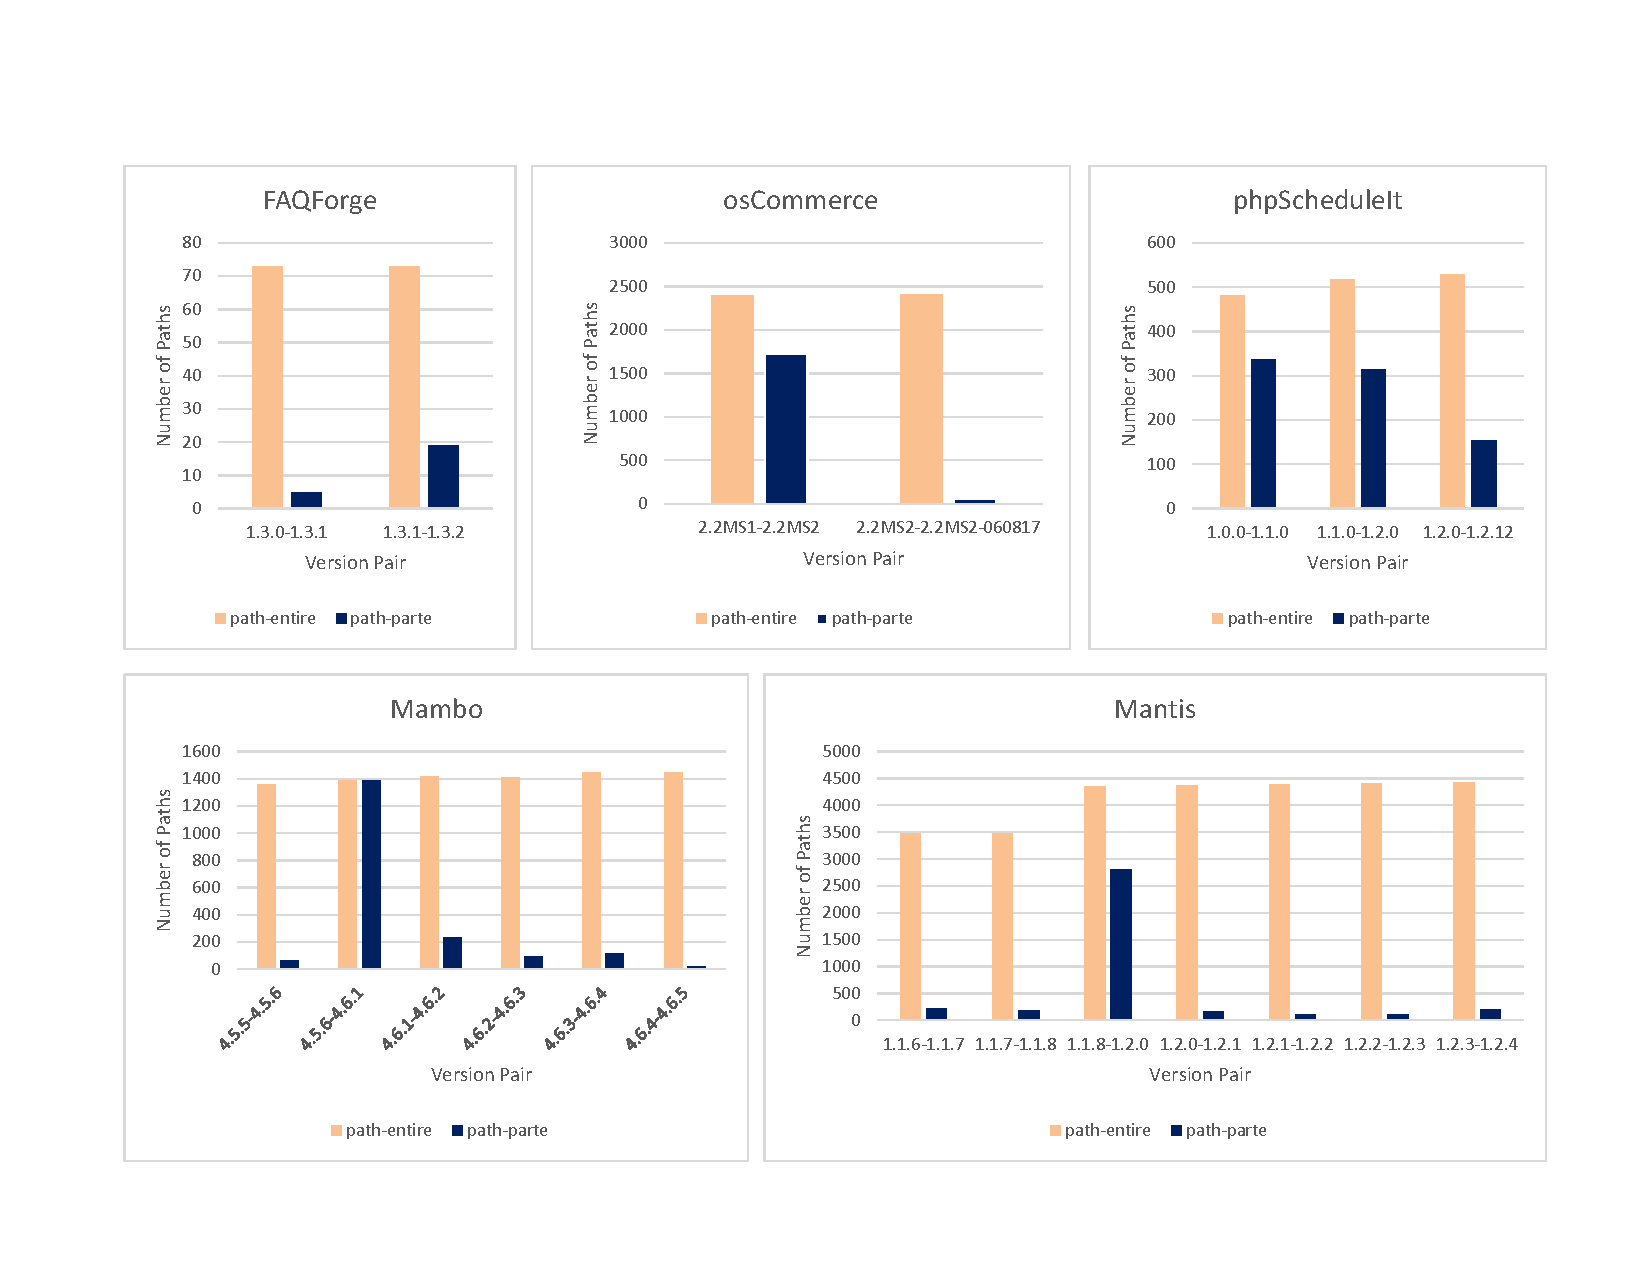
\includegraphics[width=1.0\columnwidth]{figures/bargraph.pdf}
%\leavevmode \epsfxsize=1.0\columnwidth
%\epsfbox{figures/bargraph.eps}
\vspace*{-15pt}
\caption{Experiment Results: The Total Number of Test Paths
Generated by Control and PARTE techniques}
\vspace*{5pt}
\label{fig:bargraph}
\vspace*{5pt}
\end{figure*}

\subsection{Test Input Constraints}

Because the test paths require actual inputs to create executable
test cases, by reducing the number of test paths necessary with the
modified program, we expect to produce further savings for the costs
associated with collecting test input constraints and resolving
constraints.
By automating the constraint resolution process for the majority
of inputs, we could reduce a substantial amount of time and effort
for resolving constraints manually.

To provide some ideas about how much time we can save with automatic
constraint resolution, we investigated the time taken to assign
actual values to the input variables obtained by our constraint collector.
We examined two cases from {\em osCommerce} that contain multiple numeric
and string inputs. One case has 16 inputs (2 numeric and 14 string),
and the other case has 10 inputs (2 numeric and 8 string).
To resolve all input values, it took 15 and 20 minutes, 
respectively. The tester had to go through the source files and the 
application database to figure out the proper values for them.
When we applied our tool, for the entire version of {\em osCommerce},
it took less than 5 minutes.
The input values assigned by human testers could be more realistic,
but when the number of inputs is prohibitively large to be resolved 
manually, automatic resolution would be the viable solution.
Not all inputs can be resolved with the automatic resolution tool, but
still, it would provide a good baseline that testers can utilize.

\subsection{Security Implications}

There are some security implications for this approach.
Through the experiment, we observed that the applications we 
used contained many security fixes and added security features,
and we also observed that test cases generated with our approach 
could help testers verify that a security patch or fix has been 
properly implemented.

In {\em FAQForge}, there was a security patch implemented 
between versions 1.3.1 and 1.3.2. Our test generating tool 
discovered the difference and generated several test cases 
that traversed these changes. For version 1.3.1, changes 
were made to the file that contains code for a login page that 
allows the administrators to perform security associated tasks. 
The change made to this file was the introduction of an HTML meta 
tag with an http-equiv attribute. 
This allows the page to load in all major browsers. Because the 
change happens in the header, it is important to test all code 
paths for the login page such as page load, validate username 
and password, and count failed login attempts. The test paths generated 
in our experiment include all these code paths or blocks.

In {\em osCommerce}, a similar scenario occurred between versions
2.2MS1 and 2.2MS2. The developers added some security features for 
website administration. For example, features for supporting SSL 
validation and forcing cookie usage were implemented.
Another interesting security related feature was added to
version 2.2MS2. This feature allowed users to inject shell commands 
into the web server. Our tool generated several test cases that 
covered this change. 
However, without proper inputs for these test
cases, we were not able to test this security feature correctly.
Because our current constraint resolution tool does not generate 
malicious inputs, we used our previous tool~\cite{marback09} to
generate malicious inputs. With these inputs, our tool was able 
to reveal this particular security vulnerability.
In version 2.2MS2-060817, only a few minor security fixes were made. 
For example, the fix prevented a session ID from being passed in 
Tell-A-Friend E-Mails. This fix was a minor change to the statement 
that prepares the body of the email to be sent. 
Also, there was a security fix that corrected 
an SQL injection problem between versions 2.2MS2 and 2.2MS2-060817. 
Our tool was able to generate test cases
that exercised all these fixes. 

In the case of {\em phpScheduleIt}, version 1.2.0 introduced a security 
feature where application administrators can grant permissions 
to other users. These permissions provide users the access to make, 
modify, or delete an existing reservation. Also, administrators can 
remove permissions to prevent users from accessing a resource. 
The regression tests for this version should cover code that was added 
to enable user profile management. The results from our experiment show 
that the new code blocks associated with new security features and fixes 
were included in the regression test paths generated. 

In version 4.6.2 of {\em Mambo}, a security fix was introduced. 
One such fix is about the Captcha (completely automated public 
turing test to tell computers and humans apart) feature. 
If a session is not initiated, then it is regenerated, and a new 
session code is assigned to the Captcha code. 
This produces new challenge text and audio for verification. 
Given the type and location of this fix it is important to cover all 
viable paths in this code. All these code blocks were included 
in the regression paths generated in our experiment.
 
In the case of {\em Mantis}, the version pair 1.1.6 and 1.1.7
contained one security bug fix. The fix for this bug required 
changes to the files that handle logging out of the current session 
and reloading the verification page. 
These changes impacted the blocks of code that perform logout, 
initialize a new session, and validate user credentials.
Another version pair, 1.1.8 and 1.2.0, contained one security fix. 
The bug was about the possibility of a cross site scripting attack 
through permalink\_page.php. The fix was to check if the input URL 
is safe. Because this change happened at the root level, all paths 
in the permalink\_page.php file should be included to test the fix,
and our tool was able to generate those paths. 
 
\subsection{Limitations}
\label{sec:limitations}

Although our approach and empirical results are promising,
our approach has some limitations that we want to address. 
One limitation involves test oracles. As we mentioned
in Section~\ref{sec:method}, in this work, we focused
on generating test cases, and our approach does not generate
the oracles. Automating test oracle generation or verification 
of the results could be investigated in the future. 
 
Another limitation involves test case execution.
To execute test cases automatically, the test execution engine 
needs to pass the web elements to Selenium along with test paths and
input values. However, the current path generator does not 
provide web elements, so we had to provide them manually.
As a result, we were not able to run all test cases that 
we generated through our tool. However, this issue has been identified,
and the feature addition is being developed. 
 

\section{Threats to Validity}
\label{sec:validity}

The primary threat to validity of this study is the amount of
user session data and the type of users who participated in this
study. For the private application that we used in this study,
we collected user interaction data for a long period time; 
the collected data was created by actual users of 
the application. However, for the two open source applications, 
the period of time that we collected user interactions was relatively 
short, and the participants were not domain experts or regular users 
of the applications so their usage patterns had wide variations.
This threat can be addressed by performing additional studies that
monitor user interactions over a longer time period among a wider population,
by considering industrial applications and different types of 
applications (e.g., mobile applications).
 
Another threat to validity is the choice of algorithms that classify 
components' frequency access ranking and analyze change impact. 
In this study, we applied various algorithms to create our classification
model, but many other classification algorithms (e.g., decision tree and
apriori algorithms) are available, and they could produce different results.
The results can vary depending on the type of classification algorithms, 
the parameters set for classification algorithms, the variables being analyzed, 
and the environmental settings. 

There is another concern regarding the bug reports that we used.
Our classification prediction values for designing linear models 
in the change impact analysis were generated from bug history that 
was reported by actual users.
Further, using these bug reports, we measured the coefficient of other 
variables to create our linear model for change impact analysis.
Because our bug report data is not comprehensive and contains 
only those bugs accrued 
until the time that we stopped collecting data, 
and because there might 
be other bugs that have not been reported yet or that might occur 
later, there is a possibility that the bug reports are biased.


\section{Related Work}
\label{sec:related-work}

In this section, we discuss studies of  regression testing focusing on 
test case prioritization techniques that are most closely 
related to our work. Further, we discuss recommender systems 
and research related to that topic.

\subsubsection*{Test Case Prioritization}
Test case prioritization techniques reorder test cases to maximize
some objective functions, such as detecting defects as early as possible.
Due to the appealing benefits of test case prioritization in practice, 
many researchers and practitioners
have proposed and studied various test case prioritization 
techniques. For example, these techniques help engineers discover faults
early in testing, which allows them to begin debugging earlier.
In this case, entire test suites may still be executed, which avoids 
the potential drawbacks associated with omitting test cases. 
Recent surveys ~\cite{catal13, marksurvey} provide a comprehensive 
understanding of overall trends of the techniques and suggest areas for improvement.

Depending on the types of information available, various test case
prioritization techniques can be utilized, but 
the majority of prioritization techniques have used source code
information to implement the techniques.
For instance, many researchers have utilized code coverage information
to implement prioritization techniques~\cite{elbaum02feb, kim02may,rothermel01oct}. Although this approach is simple and na\"ive, many empirical
studies have shown that this approach can be effective~\cite{cost3, 
	cost1, Malishevsky02, myra}.
Recent prioritization techniques have used other
types of code information, such as slices~\cite{jeffrey06sep}, change
history~\cite{sherriff07}, code modification information, and fault
proneness of code~\cite{mirarab07}.

More recently, several prioritization techniques 
utilizing other types of information have also been proposed. 
For example, Anderson et al.  applied telemetry data to compute fingerprints 
to extract usage patterns and for test prioritization~\cite{jeff16}.
Memon and Amalfitano performed a study in which they applied telemetry 
data to generate usage pattern profiles~\cite{memongui}.  
In another study, Amalfitano et al. built finite state models
based on usage data that they collected from rich Internet applications ~\cite{rich}. 
Carlson et al.~\cite{ryan} presented clustering-based techniques that
utilize real fault history information including code coverage.
Anderson et al.~\cite{jeff14} investigated the use of various code features
mined from a large software repository to improve regression testing techniques.
Gethers et al. presented a method  that uses textual change of source code
to estimate an impact set ~\cite{kagdichange}. 

\subsubsection*{Context-aware Recommender system}
Recommender systems are software engineering tools that make 
the decision making process easier by providing a list of relevant items.
There are three primary  categories in recommender systems:
content-based algorithms, collaborative filtering algorithms, and hybrid approaches ~\cite{recomsurvey05}.  
Recommender systems are commonly used by users in their daily routines, 
helping in such tasks as finding 
their target items more easily.
Some widely-used applications that provide recommender systems
are Amazon, Facebook, and Netflix. These applications provide suggestions
to target users based on the user or item characteristic similarities.  

Further, in the area of software engineering, due to the decline in hardware 
facility prices, a variety of information is collected by software 
providers, such as change history, issue reports and databases, user log files, 
and so on.
With the fast growth of such information, machine learning technologies  
motivate software engineers to apply recommendation systems in software 
development. Recommender systems in software engineering have been applied  
to improve software quality and to address the challenges of development process~\cite{rssebook}.  
For instance, Murakami et al. ~\cite{murakami} proposed a technique that 
uses user editing activities  detecting code relevant to existing methods. 
Christidis et al. ~\cite{costas} implemented a recommender system 
to display developer activities by using information artifacts with quantitative metrics. 
Danylenko and Lowe provided a context-aware recommender system 
to automate a decision-making process for determining the efficiency of 
non-functional requirements ~\cite{contextawar}.

As we discussed briefly, there are many types of information available 
for implementing test case prioritization techniques.
In this research, we collected over 2,000 user sessions from 
three different web applications and gathered the change history of each application. 
Our research seeks to apply item-based collaborative filtering algorithms 
to generate a recommendation list of test cases for 
test prioritization.
To our knowledge, our recommender system-based prioritization technique is novel 
and has not yet been explored in the regression testing area.



% add more content about context aware recom sys







\section{Conclusions and Future Work}
\label{sec:conclusions}

%In this paper, we presented a new regression test case
%generation approach that creates test cases using
%program slices for web applications written in PHP.
%To evaluate our approach, we conducted a controlled experiment
%using five non-trivial and open source web applications with 
%multiple versions, and the results showed that our approach can 
%be effective in reducing the number of test paths necessary for 
%the modified application by focusing only on the areas affected 
%by the modified code. 
%
%While our approach can reduce the amount of time needed to apply
%regression testing for patched web application software, it can 
%also reduce time and effort as well as improve testing effectiveness 
%when the major releases are tested because new test cases and other 
%associated artifacts are accumulated over time.
%
%The results of our studies suggested several avenues for future work.
%First, we evaluated our approach utilizing five widely used open source
%web applications. Because our approach provided promising results,
%the next natural step is to perform additional studies that apply 
%our approach to industrial contexts (e.g., using industrial-sized 
%applications or considering constraints imposed by an industry's 
%regression testing practice) to see whether our approach can address 
%an industry's practical problems. 
%
%Second, in this work, we did not consider the use of the existing test cases.
%However, by utilizing existing test cases when we test the modified program,
%we can achieve additional savings. Thus, we plan to investigate test case
%selection approaches that choose test cases that exercise the modified
%areas of code to help reduce the cost of generating new tests.
%
%Third, as we discussed earlier, resolving constraints 
%could require a lot of time and effort. 
%Thus, we plan to develop a technique that identifies reusable
%constraint values for regression test cases from the previous version
%to accommodate further savings for regression testing the web applications 
%that require frequent patches and short regression testing cycles.
%

%
\subsection*{Acknowledgments}

This work was supported, in part, by NSF CAREER Award
CCF-1564238 to University of North Texas.



\balance
\bibliographystyle{plain}
\bibliography{paper}

\end{document}
